% 繁星间漫步,陆巍的博客
\documentclass[UTF8,a5paper]{ctexart}
\usepackage{tikz}% 绘图支持

\usetikzlibrary{arrows.meta,decorations,calligraphy}

% 设置章节标题左对齐,+=表示在原有格式上追加,如果只有=则表示完全替换
\ctexset{
  section/format += \raggedright,
  subsection/format += \raggedright,
  subsubsection/format += \raggedright,
}

% tikz图形样式定义
\tikzset{
  dot/.style = {
      draw,
      fill = white,
      circle,
      inner sep = 0pt,
      minimum size = 4pt,
  }
}

\begin{document}
\section{示例一}
\begin{center}
  \def\U{*0.033*\textwidth}
  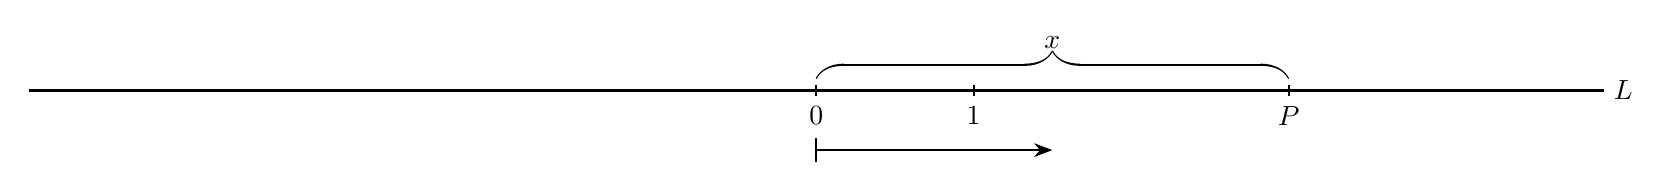
\begin{tikzpicture}[thick]
    % 绘制轴
    \draw(-10\U,0)--(10\U,0) coordinate[label={right:$L$}](xmax);
    % 绘制轴上的点
    \foreach \x/\xtext in{0/0,2\U/1,6\U/P}
      \draw[shift={(\x,0)}](0pt,2pt)--(0pt,-2pt)node[below]{$\xtext$};
    % 绘制范围括号
    \draw[decorate,decoration={calligraphic brace,amplitude=10pt}](0,1ex)
      --node[yshift=3ex]{$x$}++(6\U,0);
    % 绘制方向指示
    \draw(0,-4ex)--++(0,-2ex);
    \draw[-{Stealth}](0,-5ex)--++(3\U,0);
  \end{tikzpicture}
  
  \vspace{4ex}
  \begin{tikzpicture}[thick]
    % 绘制轴
    \draw(-10\U,0)--(10\U,0) coordinate[label={right:$L$}](xmax);
    % 绘制轴上的点
    \foreach \x/\xtext in{-6\U/P,0/0,2\U/1}
      \draw[shift={(\x,0)}](0pt,2pt)--(0pt,-2pt)node[below]{$\xtext$};
    % 绘制范围括号
    \draw[decorate,decoration={calligraphic brace,amplitude=10pt}](-6\U,1ex)
      --node[yshift=3ex]{$-x$}(0,1ex);
    % 绘制方向指示
    \draw(0,-4ex)--++(0,-2ex);
    \draw[-{Stealth}](0,-5ex)--++(-3\U,0);
  \end{tikzpicture}

  图1.1\quad 数轴
\end{center}


\section{示例二}
\begin{center}
  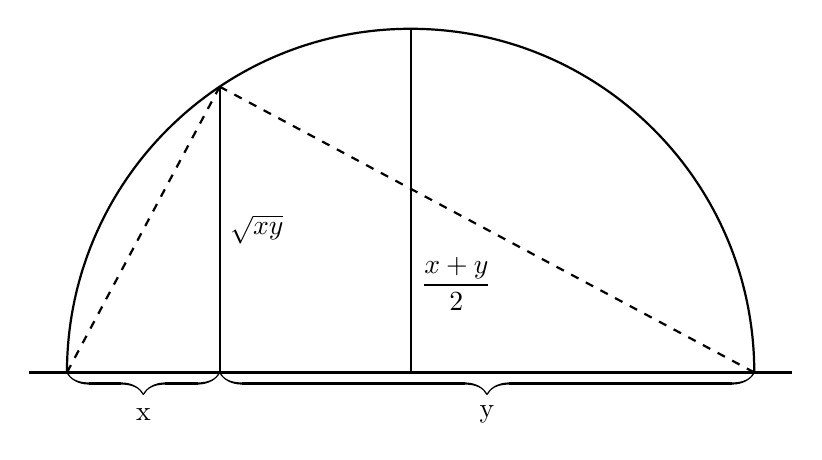
\begin{tikzpicture}[thick]
    \def\U{*0.04*\textwidth}
    \draw(-1\U,0)--(19\U,0) coordinate(xmax);
    \draw(0,0) arc[start angle=180,end angle=0,x radius=9\U,y radius=9\U];
    % 计算c点y坐标值
    \pgfmathparse{sqrt(4*14)}
    \path
      coordinate (c) at (4\U,\pgfmathresult\U);
    \draw(9\U,0)--node[yshift=-7ex,right]{$\displaystyle\frac{x+y}{2}$}++(0,9\U);
    \draw(4\U,0)--node[right]{$\sqrt{xy}$}(c);
    \draw[dashed](0,0)--++(c);
    \draw[dashed](c)--(18\U,0);
    \draw[decorate,decoration={calligraphic brace,amplitude=8pt}](4\U,0)--node[yshift=-3.5ex]{x}(0,0);
    \draw[decorate,decoration={calligraphic brace,amplitude=8pt}](18\U,0)--node[yshift=-3.5ex]{y}(4\U,0);
  \end{tikzpicture}
  
  图1.6\quad $x$和$y$的几何平均值和算术平均值
\end{center}



\section{示例三}
\begin{center}
  \begin{tikzpicture}[thick]
    \def\U{*0.027*\textwidth}
    % 绘制坐标轴
    \draw[-{Stealth}](-2\U,0)--(18\U,0) coordinate[label={right:$x$}];
    \draw[-{Stealth}](0,-2\U)--(0,13\U) coordinate[label={above:$y$}];
    % 设定坐标点
    \path
      coordinate(x) at (11\U,0)
      coordinate(y) at (0,7\U)
      coordinate(c) at (11\U,7\U)
      coordinate(c1) at (7\U,5\U)
      coordinate(c2) at (15\U,9\U);
    \draw[dashed](y)--(c)--(x);
    % 绘制曲线
    \draw(7\U,5\U) cos(11\U,7\U) sin(15\U,9\U);
    % 绘制各点标签
    \draw
      (y)node[dot,label={left:$y$}]{}
      (c)node[dot]{}
      (x)node[dot,label={below:$x$}]{}
      (0,0)node[dot,label={below left:$0$}]{};
  \end{tikzpicture}
  
  图1.7\quad 函数的图形
\end{center}

\end{document}
